The User Interface, later in the text UI, has been split into two sections. One more suitable for a regular user, which contains stylized components representing our results. The other section consists of JSON REST API user interface, where data and our results are represented in JSON format. We will give more comprehensive explanation of each of them in the following two sections.

\subsection{Web Application UI}

In this section we have shown data from the data dump such as list of posts with their related comments. Post details are shown in a separate fragment of the page shown in the figure below. Fragment consist of content of the post, post engagement and links towards Facebook post and JSON REST API web page containing same information in JSON format.

\begin{figure}[ht]
	\centering	
	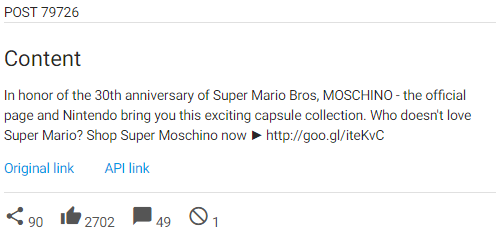
\includegraphics[width=1\textwidth]{04-framework/03-user-interface/images/post_details.png}
	\caption[Post Details Fragment]{Post Details Fragment \label{fig:post-details}}
\end{figure}
 
User is able to choose a specific post from the list of post located in the left side of the page. Choosing a post, fragment containing post details reloads with new data and under it lists all comments related to it. List item of the comment list is represented in next figure. Comment fragment has original language comment content and the English translated version, under the content we outlined sentiment analysis results of most accurate API compared with real sentiment score. User can see detailed representation of sentiment scores for each API separately. In case of comment being marked as spam, there is an indicator clearly pointing it out.

\newpage

\begin{figure}[ht]
	\centering	
	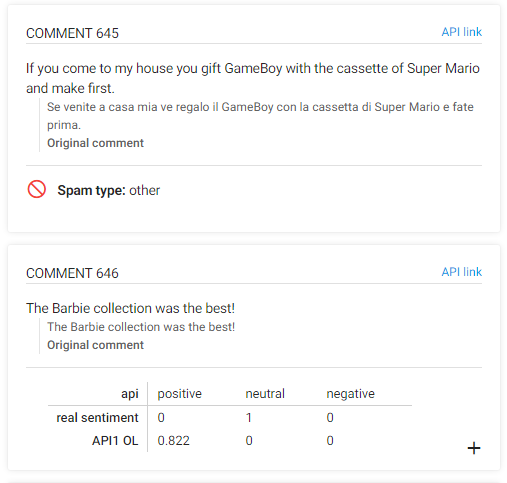
\includegraphics[width=1\textwidth]{04-framework/03-user-interface/images/comment_fragment.png}
	\caption[Comment Fragment]{Comment Fragment \label{fig:comment-fragment}}
\end{figure}

Keeping in mind that most preferred way of representing data is though visualization, we have decided to show sentiment scores though pie charts. Fragment that contains the chart is located on the right side of the web page. The chart fragment contains two pie charts, one representing statistics related to real sentiment score and second representing statistics related to sentiment score of chosen API as shown in the figure 4.5. User is able to choose between different API in order to visually compare them with real sentiment scores.

\newpage

\begin{figure}[ht]
	\centering	
	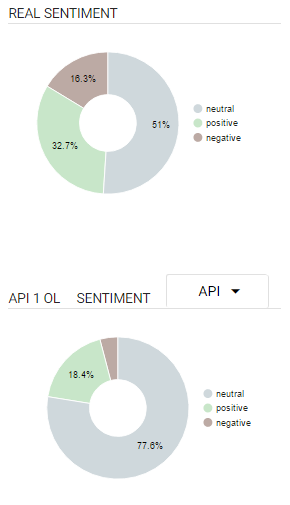
\includegraphics[width=0.5\textwidth]{04-framework/03-user-interface/images/pie_chart.png}
	\caption[Chart representation of sentiment score]{Chart representation of sentiment score \label{fig:pie-fragment}}
\end{figure}

Navigation to Stats tab, we are showing how we have calculated the accuracy of APIs, listed how many samples we have conducted the research on and listed percentage of negative, positive and neutral real sentiment comments. This webpage is giving opportunity to the user to see tabular representation of statistical results of each API with or without emojis, API with data translated in English and results taking into consideration the spam filters. Such tabular view has been enclosed below this paragraph. 

\begin{figure}[ht]
	\centering
	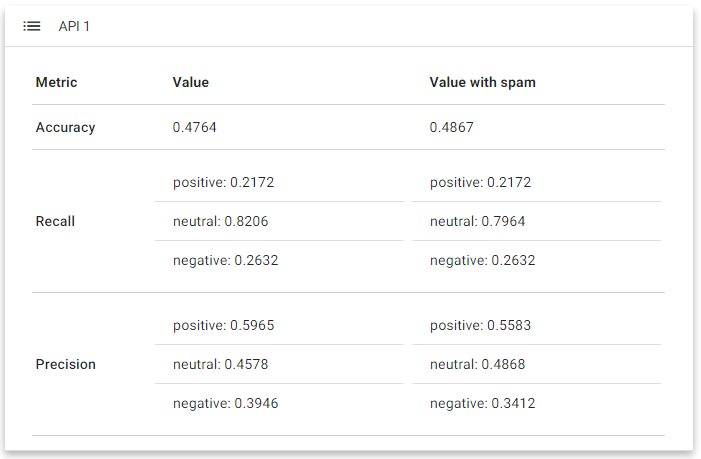
\includegraphics[width=0.8\textwidth]{04-framework/03-user-interface/images/stats.png}
	\caption[Tabular representation of statistical results for an API]{Tabular representation of statistical results for an API \label{fig:stats}}
\end{figure}

\newpage

\subsection{JSON REST API UI}

This section represents the data in JSON form using Django REST Framework. The used framework has brought us to having a browsable Web API in few steps. Following official documentation we were able to define all the relations between our entities and easily retrieve needed data. One of few views we are able to reach is shown on the figure below.

\begin{figure}[ht]
	\centering
	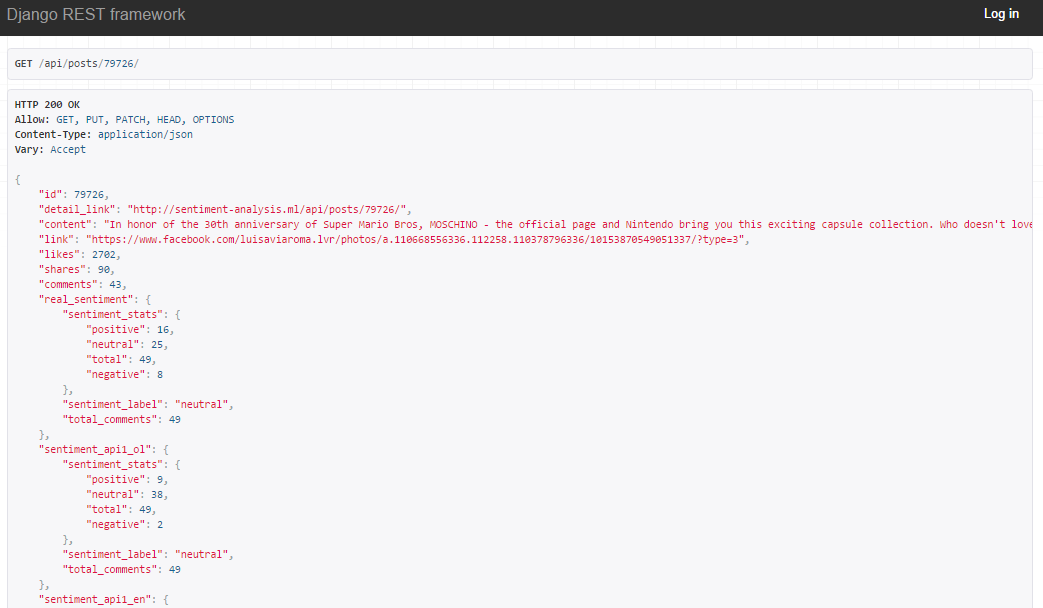
\includegraphics[width=0.8\textwidth]{04-framework/03-user-interface/images/django_api.png}
	\caption[JSON representation]{JSON representation \label{fig:django-api}}
\end{figure}